\documentclass{report}
\usepackage{a4}
\usepackage{hyperref}
\usepackage{graphicx}
\usepackage{listings}
\usepackage{tabularx}
\usepackage{pifont}
\usepackage{algorithm}
\usepackage{algpseudocode}
\usepackage{amsmath}
\usepackage{amssymb}
\usepackage{amsthm}
\usepackage{fixltx2e}
\usepackage{graphics}
\usepackage{graphicx}
\usepackage{program}
\usepackage[english]{babel}
\usepackage[T1]{fontenc}
\usepackage[english]{babel}
\usepackage{amsmath,amssymb,amsfonts,textcomp}
\usepackage{color}
\usepackage{calc}
\usepackage{longtable}
\usepackage{amssymb}
\newcommand\textstyleTeletype[1]{\texttt{#1}}


\begin{document}

\title{Exploring Machine Learning:\\
  The ID3 algorithm\\
  		Narrative and Reflective Document}


\author{Mohammed Ibrahim\\
 Computer Science Department\\
  College of Science, Swansea University\\
  Swansea, SA2 8PP, UK
}

\maketitle

\abstract{This project is based on Machine Learning. The two programs has been created to test the ID3 algorithm. The program produce the decision tree in the form of if, else clause. This report contains the project challenges and mentions possible improvements along with what we have learned from this project. }


\tableofcontents
\pagebreak

\chapter{Narrative and Reflective Document}
\label{sec:nar}


\section{Introduction}
\label{sec:intro}

The project assigned to me is based on Exploring Machine Learning using ID3 Algorithm which describe the technique and methods that involves making machine to learn and behave based on training data given and past experience to improve its performance. In this project we used the techniques of ID3 algorithm to implement and validate the \emph{Decision Tree}. To illustrate the operation of ID3 algorithm we representing the training set \ref{fig:trainingplaytennis}.To test ID3 algorithm and to implement the decision  tree we have created two Java programs. The first Java program has been implemented to create the Decision tree in the form of if and else clause. In second program we give validation set to check decision tree based on target attribute.

\section{Development Narrative}
\label{sec:dev}

The first program is an implementation of the ID3 algorithm. The first program reads the input file, \emph{training set} according to our specified file format. There will be different kinds of file formats for different kinds of information. Some file formats are designed for very particular sorts of data. The main objective of having an input file format for our program is that we need the input to be consistent every time the program runs. The input file format rules are:

\begin{enumerate}

\item Comments are ignored in the file by using double slash ($//$) symbol. 
\item Blank line also be ignored in the data file.
\item The attributes and values are separated by using single space.
\item Every file should have end of line.
\item The very first recognizable line of the data file have to be an attributes.
\item The number of attributes is inferred from the number of words in this line.
\item The last word of the attributes is taken as the {\emph target attribute. }
\item In the data file each subsequent line contains the values of attributes for a data point.
\end{enumerate}

The first program was developed by using some techniques from existing program which was developed by Dr.Benny Raphael\cite{ID3Algorithm}.I used similar types functions which will return the value of attributes by calculating entropy \cite{ID3Algorithm} and I have also used decompose node function \cite{ID3Algorithm} which will specify the node according to ID3 algorithm. The first program also output the size of the complete table.

The two programs was developed to test the ID3 algorithm. As an individual enjoyed working in Java programming language. During the first phase I found difficult to start writing programs, with the help of my supervisor I understand the clear concept of both the programs.\\
In phase two we have created second program to implement the output of the id3 algorithm (decision tree) in the \emph{tennis example data set}. Then this program tested on validation set that we created for this purpose.The validation set does include the target attributes, however the program will not read that attribute. The second program has been written in a such a way that the program reads the validation set and output the the predicted attribute. 
The program will compare each predicted output with actual target value and it counts how many example being wrongly predicted and calculate the percentage rate.This is very useful measure\emph{(error rate)} to indicate how accurate is the decision tree. 



\pagebreak

\subsection{Entropy}
\label{sec:inf}

\textbf{Entropy} is one kind of measurement procedure in information theory which will characterize the impurity of an arbitrary collection of examples. Entropy measures the amount of information in attribute and It is also called measure of unpredictability. \\
Here, we will calculate Entropy from the set of data given in training set \emph{play tennis} \ref{fig:trainingplaytennis}

\textbf{ The formula for calculating the entropy \cite{Mitchell1997MachineLearning}(Chapter3, page 56) :}\\

{\centering
 $\mathit{Entropy}(S)=-p_\oplus\log _{2}p_\oplus - p_\ominus\log _{2} p_\ominus$ 
\par}

Where,

\begin{itemize}

\item \textbf{`S'} containing positive and negative examples of some target concept.
\item The entropy of \textbf{`S'} relative to boolean classification. i.e
\item $\mathit{p_\oplus}$ is the proportion of positive examples in \textbf{`S'}. 
\item $\mathit{p_\ominus}$ is the proportion of negative examples in \textbf{`S'}.
\item In tennis example(in target attribute) we have 9 positive proportion and 5 negative proportion .  ( i.e boolean value : play = Yes or No).
\item The \textbf{Entropy} specifies the minimum number of bits of information need to encode the classification of an arbitrary member of \textbf{`S'}.

\end{itemize}

If S is a collection of 14 examples with 9 YES and 5 NO examples then\\

{\centering
$\mathit{Entropy}(S) = {}- (9/14) Log{2} (9/14) {}- (5/14) Log{2} (5/14) = 0.940$
\par}

Notice entropy is 0 if all members of \textbf{`S'} belong to the same class (the
data is perfectly classified). \\


\begin{itemize}

\item If all target values that are associated with the attribute  are positives or negatives then the entropy is equals 0.
\item If the examples associated with certain attributes contains equal number of positives and negatives then the entropy equals 1.

\item if the target values that are associated with the attribute are both positives and negatives then the entropy for that attribute will be between 0 and 1.
\end{itemize}
\pagebreak

For a general case where the target classification is not boolean, then the target attribute can take on \emph{`c'} different values. Then the entropy of \emph{`S'} that is associated with \emph{`c'} classes calculated as :

{\centering
 $\mathit{Entropy}(S)=\sum\limits_{i=1}^c-p_i\log _{2}p_i$ 
\par}

\begin{itemize}

\item Where, \textit{p(i)} is the proportion of S belonging to class \textit{i} .
\item $\mathit{\sum }$ is over \textit{c} . $\mathit{\log_{2}}$ is log base 2.

\end{itemize}

Now we have calculate the measure of the effectiveness of an attribute in classifying the training data, the measure which we use is called as \texttt{information gain}.

More clearly, the information Gain(S, A) is information gain of example set S on attribute A is
defined as:\\

{\centering

Gain(S, A) = $\mathit{Entropy}(S)=\sum\frac{S_v}{S} Entropy (S_v)$


\par}

Where:

${\Sigma}$ is each value v of all possible values of attribute A

S\textsubscript{v} = subset of S for which attribute A has value v

{\textbar}S\textsubscript{v}{\textbar} = number of elements in
S\textsubscript{v}

{\textbar}S{\textbar} = number of elements in S\\


Suppose,
\begin{itemize}

\item S is a set of 14 examples in which one of the attributes is called \emph{wind} .
\item The values of Wind can be \textit{Weak} or \textit{Strong}. 
\item The classification of these 14 examples have  9 \emph{YES} and 5 \emph{NO} . 
\item For attribute Wind, suppose there are 8 occurrences of Wind = Weak and 6 occurrences
of Wind = Strong. 
\item For Wind = Weak, 6 of the examples are YES and 2 are NO. For Wind = Strong 3 are YES and 3 are NO.\\ 
\end{itemize}
\pagebreak

\subsection{Information Gain Calculation}
\label{sec:inf}

Information gain is the procedure to select a specified or particular attribute to be a decision node of a decision tree.

{\bf (Wind)}

$\mathit{Entropy}(S\textsubscript{weak}) = \textstyleTeletype{{}-} (6/8)*\log_{2}(6/8)
{}- (2/8)*\log{2}(2/8) = 0.811$

$\mathit{Entropy}(S\textsubscript{strong}) = \textstyleTeletype{{}-}
(3/6)*\log{2}(3/6) {}- (3/6)*\log{2}(3/6) = 1.00$\\

{\centering
\textstyleTeletype{Gain(S,Wind)=Entropy(S){}-(8/14)*Entropy(S}\textsubscript{weak}\textstyleTeletype{){}-(6/14)*Entropy(S}\textsubscript{strong}\textstyleTeletype{)}
\par}

\textstyleTeletype{= 0.940 {}- (8/14)*0.811 {}- (6/14)*1.00}

\textstyleTeletype{= 0.048}\\

So, the information Gain of wind over `S' is 0.048. In the book of Mitchell it shows the calculation for single attributes \cite{Mitchell1997MachineLearning}.\\
Using the same procedure we calculated information gain for other attributes such as : Outlook, temperature and humidity.  Based on the ID3 Algorithm we select the Outlook attributes because it has highest gain, therefore it is used as the decision attribute in the root node.

{\bf (Humidity)}

$\mathit{Entropy}(S\textsubscript{High}) = \textstyleTeletype{{}-} (3/7)*\log_{2}(3/7)
{}- (4/7)*\log{2}(4/7) = 0.985$

$\mathit{Entropy}(S\textsubscript{Normal}) = \textstyleTeletype{{}-}
(6/7)*\log{2}(6/7) {}- (1/7)*\log{2}(1/7) = 0.592$\\

{\centering
\textstyleTeletype{Gain(S,Humidity)=Entropy(S){}-(7/14)*Entropy(S}\textsubscript{High}\textstyleTeletype{){}-(7/14)*Entropy(S}\textsubscript{Normal}\textstyleTeletype{)}
\par}
\textstyleTeletype{= 0.940 {}- (7/14)*0.985 {}- (7/14)*0.592}

\textstyleTeletype{= 0.151}\\

{\bf (Temperature)}

$\mathit{Entropy}(S\textsubscript{Hot}) = \textstyleTeletype{{}-} (2/4)*\log_{2}(2/4)
{}- (2/4)*\log{2}(2/4) = 1$

$\mathit{Entropy}(S\textsubscript{mild}) = \textstyleTeletype{{}-}
(4/6)*\log{2}(4/6) {}- (2/6)*\log{2}(2/6) = 0.918$\\

$\mathit{Entropy}(S\textsubscript{cool}) = \textstyleTeletype{{}-}
(3/4)*\log{2}(3/4) {}- (1/4)*\log{2}(1/4) = 0.811$\\

{\centering
\textstyleTeletype{Gain(S,Humidity)=Entropy(S){}-(4/14)*Entropy(S}\textsubscript{High}\textstyleTeletype{){}-(6/14)*Entropy(S}\textsubscript{Normal}\textstyleTeletype{)}
\par}
\textstyleTeletype{= 0.940 {}- (4/14)*1 {}- (6/14)*0.918{}-(4/14)*0.811}

\textstyleTeletype{= 0.029}\\



{\bf(Outlook)}

$\mathit{Entropy}(S\textsubscript{High}) = \textstyleTeletype{{}-} (2/5)*\log_{2}(2/5)
{}- (3/5)*\log{2}(3/5) = 0.971$

$\mathit{Entropy}(S\textsubscript{Normal}) = \textstyleTeletype{{}-}
(3/5)*\log{2}(3/5) {}- (2/5)*\log{2}(2/5) = 0.971$\\

{\centering
\textstyleTeletype{Gain(S,Humidity)=Entropy(S){}-(7/14)*Entropy(S}\textsubscript{High}\textstyleTeletype{){}-(7/14)*Entropy(S}\textsubscript{Normal}\textstyleTeletype{)}
\par}
\textstyleTeletype{= 0.940 {}- (5/14)*0.971 {}- (5/14)*0.971}

\textstyleTeletype{= 0.246}\\

For each attribute, the gain is calculated and the highest gain is used
in the decision node.

We consider the tennis example and we apply the ID3 algorithm to check all the 4 attributes.
When we consider the first step from the ID3 algorithm, the top most node of the decision tree was created. To know which attribute to test first, ID3 algorithm determines the information gain for each candidate attribute. 

\begin{itemize}
\item Outlook
\item Humidity
\item Wind
\item Temperature
\end{itemize}
\pagebreak
From the calculation of information gain measure, we say that the \emph{outlook} attribute provides the best prediction of the target attribute, ( \emph{Play Tennis} ) over the tennis example data set.\\
So, we have selected \emph{Outlook} attribute as the decision attribute for the root node, the branches are created for each of its possible values such as : (\emph{sunny, overcast, rain}).
In the below tennis example which \emph{outlook = overcast} is also a positive example of \emph{play tennis}, therefore this node of the tree becomes a leaf node with classification \emph{PlayTennis}. The other attributes such as \emph{Outlook=sunny and Outlook=rain} still have nonzero entropy, and the decision tree will be further elaborated below these nodes.\\

The main idea here is to get a new attribute and check if the attribute has been selected in higher level of the tree or not. if it has been incorporated in the higher level of the tree then it will be excluded, otherwise it will be consider and then calculate entropy for that attributes with respect to the example that are associated with it.\\
This process will be repeated for each non-terminal descendant node and the attribute will be a terminal node {leaf node} if it's entropy = 0 , no more attributes to be considered.

\pagebreak

According to \cite{Mitchell1997MachineLearning}(page 59,Chapter 3): Training set : In machine learning training sets are generally called as tables, where each row in the table represents a single training example. 

To illustrate the operation of ID3, we consider the learning task represented by the example training set given in Figure \ref{fig:trainingplaytennis} We have four attributes Outlook, Temperature, Humidity and Wind. The target attribute is called PlayTennis, which has values boolean value \texttt{yes} or \texttt{no} for different Saturday mornings, is to be predicted based on other attributes of the morning in question. 
\begin{figure}[h]
  \centering
  \begin{tabular}{|c|l|l|l|l|l|l|}
    \hline
    Day & Outlook & Temperature & Humidity & Wind & PlayTennis\\
    \hline
    1 & sunny & hot & high & weak & no
    \\\hline
    2 & sunny & hot & high & strong & no
    \\\hline
    3 & overcast & hot & high & weak & yes
    \\\hline
    4 & rain & mild & high & weak & yes
    \\\hline
    5 & rain & cool & normal & weak & yes
    \\\hline
    6 & rain & cool & normal & strong & no
    \\\hline
    7 & overcast & cool & normal & strong & yes
    \\\hline
    8 & sunny & mild & high & weak & no
    \\\hline
    9 & sunny & cool & normal & weak & yes
    \\\hline
    10 & rain & mild & normal & weak & yes
    \\\hline
    11 & sunny & mild & normal & strong & yes
    \\\hline
    12 & overcast & mild & high & strong & yes
    \\\hline
    13 & overcast & hot & normal & weak & yes
    \\\hline
    14 & rain & mild & high & strong & no
    \\\hline
  \end{tabular}
  \caption{Training set for \texttt{PlayTennis} example}
  \label{fig:trainingplaytennis}
\end{figure}



\subsection{ID3 algorithm}
\label{sec:id3}

ID3 searches through the attributes of the training instances and extracts the attribute that best separates the given examples. If the attribute perfectly classifies the training sets then the ID3 stops; otherwise it recursively operates on the m (where m = number of possible values of an attribute) partitioned subsets to get their "best" attribute.
The ID3 algorithm given from the book of \cite{Mitchell1997MachineLearning}(Chapter 3, page 56):
\begin{itemize}
\item Examples : are the training examples \ref{fig:trainingplaytennis}
\item target-attribute : is the attribute whose value is to be predicted by the tree.
\item Attributes : is a list of other attributes that may be tested by the learned decision tree.\\
Returns a decision tree that correctly classifies the given examples.\\
\end{itemize}


\begin{tabbing}
Create a root node for the tree\\
If \= all examples are positive, Return the single-node tree Root, with label = +.\\
If \= all examples are negative, Return the single-node tree Root, with label = -.\\
If \= Attributes is empty, Return the single-node tree Root, with label = most common value of\\ target attribute in Examples\\
Otherwise Begin \\
\> then \=  A = The Attribute that best classifies examples.\\
\> Decision Tree attribute for Root = A.\\
\> For each possible value, vi, of A,\\
\> \> Add a new tree branch below Root, corresponding to the test A = vi.\\
\> \> Let Examples(vi) be the subset of examples that have the value vi for A\\
\> \> If Examples(vi) is empty\\
\> \> Then below this new branch add a leaf node with label = most\\
\> \> common target value in the examples\\
\> \> Else below this new branch add the subtree ID3 \\
\> \> (Examples(vi), target attribute, Attributes – {A})\\

end\\
return Root\\
\end{tabbing}



\pagebreak

\subsection{Decision Tree}
\label{sec:dec}

The Decision tree for the above tennis example \ref{fig:trainingplaytennis} in the form of if,else clause and I have also included the Decision tree in the form of graphical representation that will show the root node, branches and leaf node according to tennis example \ref{fig:trainingplaytennis}.
\begin{lstlisting}

if( outlook == "sunny") {
	if( humidity == "high") {
			play = "no";
	} else 	if( humidity == "normal") {
			play = "yes";
	}
} else if( outlook == "overcast") {
		play = "yes";
} else if( outlook == "rain") {
	if( wind == "weak") {
			play = "yes";
	} else 	if( wind == "strong") {
			play = "no";
	}
}

\end{lstlisting}

\begin{figure}[hbtp]
\centering
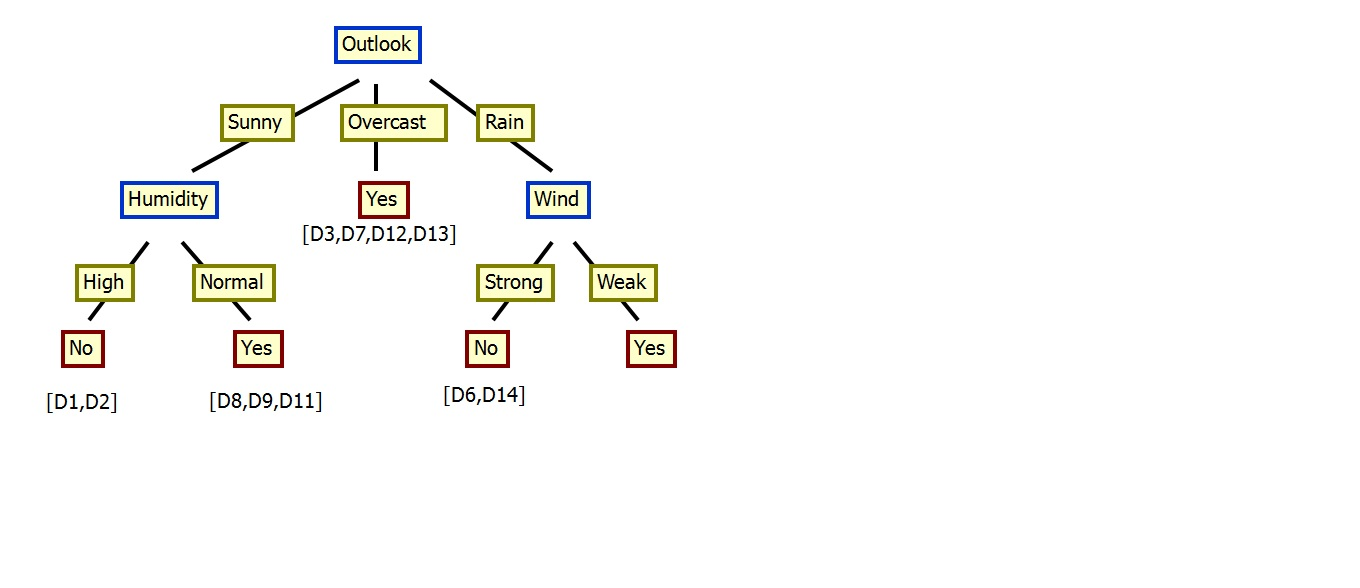
\includegraphics[width = 10in]{DecisionTree.jpg}
\caption{Decision Tree}
\end{figure}

\pagebreak
To cite from \cite{Mitchell1997MachineLearning}(page 59, chapter 3): A ``decision tree'' is a special method to represent the partial training set in a complete form. Based on the bias ``good representations are short'', the heuristics construct a ``short'' decision tree. A basic heuristics is captured by the ID3 algorithm. According to \cite{Mitchell1997MachineLearning}(page 55, chapter 3) The ID3 algorithms learns decision trees by constructing them top down, each instance attribute is evaluated using a statistical test to determine how well it alone classifies the training examples. The best attribute is selected and used as the test at the root node of the tree. A descendant of the root node is then created for each possible value of this attribute , and the training examples are sorted to the appropriate descendant node. The entire process is then repeated using the training examples associated with each descendant node to select the best attribute to test at that point in the tree. 

Explanation of decision trees: To refer from \cite{Mitchell1997MachineLearning}(page 52, chapter 3): The decision tree defines the unique path from the root of the tree to some leaf node, which provides the classification of the instance. Once we compute decision tree it is easy to complete the training set table. 

It returns ``positive'' or ``negative'' value based on that decision can be taken for a tested variable. At a lower level decision trees can be also be represented in the form of if-then rules that can be easily understand.


According to \cite{Mitchell1997MachineLearning}(page 52,chapter 3): Decision tree classifies in the form of tree structure where each branch node represents a choice between a number of alternatives, and each leaf node represents a decision. Decision tree mainly classify data using attributes and it consists of decision nodes and leaf nodes. The tree has number of branches representing with the tested attribute values. Leaf node attribute generate uniform result and it doesn't require any additional classification testing. A leaf node indicates the value of target attribute where as a decision node states some test which can be carried out on single attribute-value, with one branch and sub-tree for each possible outcome of the test.

Decision Tree classify instances by sorting them down the tree from the root to some leaf node, which provide the classifications of the instances, Each node in the tree specifies a test of some attribute of the instances and each branch descending.
Decision tree are commonly used for obtaining information for the purpose of decision making. The tree starts with root node then user split each node recursively according to decision tree learning algorithm.
According to \cite{Mitchell1997MachineLearning}(page 52, chapter 3): Decision tree learning is a method for approximating discrete-valued target functions, in which the learned function is represented by a decision tree. Decision tree learning is one of the most widely used and practical methods for inductive inference. The 3 widely used decision tree learning algorithms are: ID3, ASSISTANT and C4.5. Based on research have decided to do an implementation on ID3 algorithm. 


\pagebreak

\subsection{First Program}
\label{sec:fp}


The development of the first program started from the beginning of January 2012. The program reads the training set file and output the decision tree in a separate file. We have specified the input file format. The program reads the training set file according to specified file format, there are basically two two types of files such as valid and invalid file.\\
The program only reads the valid training set file and if we input any invalid file the program gives an error. The file format will be discussed in the below section.\\

I will be explaining briefly how the two programs work. 
In first program we have three classes {\bf FirstProg, Data, TNode}.

\begin{itemize}

\item FirstProg : Inside this class we have two subclass, one constructor and all the functions.
\item Data : This class represent a data consisting of attr values of attributes.
\item TNode : This class represents a node in the decomposition tree. It deals with one node at a time.
\end{itemize}


I will be describing each and every function which included in the first program. 
 
\begin{itemize}

\item {\bf getAttributeValue()}  This function has two parameters and it returns integer corresponding to symbolic value of attributes.

\item {\bf []getAllValues()} This function has two parameters and this function returns the values of specified attribute in the data set.

\item {\bf getSubset()} This function has three parameters and it returns the subset of data.

\item {\bf calculateEntropy()} This function has only one parameter such as :\emph{set} and it calculate the entropy of the set data points. The entropy is calculated using the values of the output attribute that is the last elements in the array attributes. 

\item {\bf DecompTree()} This function has two parameters and it checks if the specified attribute is used to decompose the data set in any of the parent\_nodes of the specfied node in the decomposition tree. It Recursively checks the specified node as well as all parent\_nodes.

\item {\bf decomposeNode() :} This function has only one  parameter and it decomposes the specified node according to ID3 Algorithm.

\item {\bf readData()} This function has one parameter,this function reads the training set file. The first line of the training set file have to contain all the attributes name.The number of attributes is inferred from the number of words in this line. The last attribute is taken as target(output) attribute. 

\item {\bf decisionTree()} This function has namely three parameters, this function prints the tree in form of if,else clause.
\end{itemize}
 
\subsection{Second Program}
\label{sec:sp}

The second program checks the decision tree which we produced in the first program.  My program works only for a specific training set such as :\emph{Tennis example}. \ref{fig:trainingplaytennis}
The second program reads the validation set 

The second program only output all the {\bf Target attributes}. In tennis example we have 14 possible values,

In second program we have one class and two function. 
\begin{itemize}

\item {\bf validateData()}

\item {\bf CalculateErrorRate()} This function calculate the error rate. Error rate is a simple formula to give an idea about the accuracy of the decision tree. It calculates the proportion of examples that have been misclassified by the decision tree.


\end{itemize}


\subsection{Training sets}
\label{sec:ts}

Training sets also called as data sets these sets are very essential as to test the programs. We input the different types of training sets into our program. The data sets are separated as valid and invalid data set.
If any training sets matches to our specified file format that sets we called as Valid data sets.
We also have some validation sets. Validation sets are those sets which we will create our self to check the second program by giving false values in the sets. I have also included validation sets in the folder called as `check.txt'

\section{Evaluation}
\label{sec:eva}

The evaluation is very important to test the programs.
Implementation of our training sets is evaluated, this evaluation will be able to find how often these sets are correct and how often they are not. These can be done according to our specified file format.

A training set of an unseen situation can be placed into our algorithm, which in turn will give an answer. Then we can compare whether the evaluation given is the one we wanted.
To test the algorithm we check by assuming all the answers given by giving false values. Then an example can be applied which we have read up upon from literature or case studies. the evaluation given by our algorithm can then be compared with the ones from the source document.

\section{Improvements}
\label{sec:imp}

All Machine learning projects looks very interesting and challenging, as a MEng student I feel my self bit difficult the reason is I was not aware of these topics I actually needed more time to understand the concept but it took me long time to understand as my English level is intermediate. After coming to Swansea University I have improved my writing and communication skills.  
With the help of my supervisor I understand the concept of ID3 algorithm and the implementation of Decision tree. 
This project was challenging for me to do I my self slowly started understanding the concept of ID3 algorithm. In requirements and specification document my marks was too low but I have tried my best in the interim document and have explained in a precise manner. I was not aware of {\bf Github and \LaTeX{}} while doing this project I learned how to use \LaTeX{}.

\section{Tools and Software}

\subsection{ Source control management  GIT AND GITHUB}
\label{sec:git}

Git helps users to communicate securely with remote repository at GitHub.com. It is a remote repository hosting provider with which we can share projects.	
According to \cite{Chacon2011ProGit} (page 5, chapter 1): Git is a powerful, fastest, sophisticated distributed version control system this is quickly replacing subversion in open source and corporate programming communities. It is written in C language and it is active from several years. It designed to handle extremely large projects with speed and efficiency,	but just as well suited for small personal repositories; it is especially popular in the open source community, serving as a development platform for projects like the Linux Kernel, Ruby on Rails, WINE or X.org.
Birth of GIT:
According to \cite{Chacon2011ProGit} (page 5, chapter 1): In the year 2002 Linus Benedict Torvalds uses Bit-Keeper for tracking Linux when it gets better, he writes his own Source Control Management, GIT. Later GIT officially used to track Linux and released GIT 1.5.0 version in the year 2007.I will be using 1.7.8 version.
Repository:  A repository is a set or collection of commits, the work which you have done past it shows in an archive and looks like project's working tree in your machine or someone else's. It holds a set of branches and tags, to identify certain commits by name.

The index : Git does not commit changes directly from the working tree into repository. Changes are first registered in the index,it is the way of confirming changes one by one before doing any commit.																										

Working tree :the directory in a file system called working tree which has repository by stating extension .git and it includes all the files and sub directories in that  directory.

Commit : the word "commit" is often used by git, other revision control systems use the words "version".

\subsection{\LaTeX{}}
\label{sec:lat}

This is the first time that I have used latex to write my project report.Using this program has been a highly educational experience for me. 
According to \cite{Mittelbach2004TheLatexCompanion} (page 15, chapter 2): 
 will be used for several purposes, such as writing an articles, business and personal letters or producing overhead slides.
``TEX " is a new typesetting system intended for the creation of beautiful books and especially for books that contain a lot of mathematics. The worldwide availability of ``LATEX" rapidly increased international interest in ``TEX" and in its use for typesetting a range of languages.

\section{Conclusion}
\label{sec:con}

The idea of ID3 algorithm is to produce the decision tree based on the training data set, this decision tree will be able to perform a  prediction.
ID3 searches through the attributes of the training instances and extracts the attribute that best separates the given examples. If the attribute perfectly classifies the training sets then the ID3 stops; otherwise it recursively operates on the m (where m = number of possible values of an attribute) partitioned subsets to get their "best" attribute.
Hence we say Decision Tree classify instances by sorting them down the tree from the root to some leaf node, which provide the classifications of the instances, Each node in the tree specifies a test of some attribute of the instances and each branch descending.
Decision tree are commonly used for obtaining information for the purpose of decision making. 
The ID3 is one algorithm to create the decision tree, there are other types of algorithm which will also create the decision tree. As far this project we haven't solved a real problem using ID3 algorithm to see its effectiveness and also we haven't done the comparison between this algorithm and the other algorithm.



\bibliographystyle{plain}

\bibliography{Bibliography}



\end{document}